\section{Discussion}
To establish a space of comparison with the previous work done on the subject of mapping a maze under supervisor Tor Onshus, it is beneficial to look at the previous reports and mappings done by other students. I am looking for information to help me address the points given in the problem description, such as:
\begin{itemize}
\item Can the accuracy of the characterization of the maze be improved using an image sensor?
\item Determine if there are any built in benefits of using an image sensor and image processing to map the maze?
\end{itemize}
The following Figures are setups and mapping of two different mazes done by previous students. They key points to look for here is how their system maps the maze walls, in terms of consistency and completeness, and if the walls are mapped at the correct locations.

\begin{figure}[H]
\centering
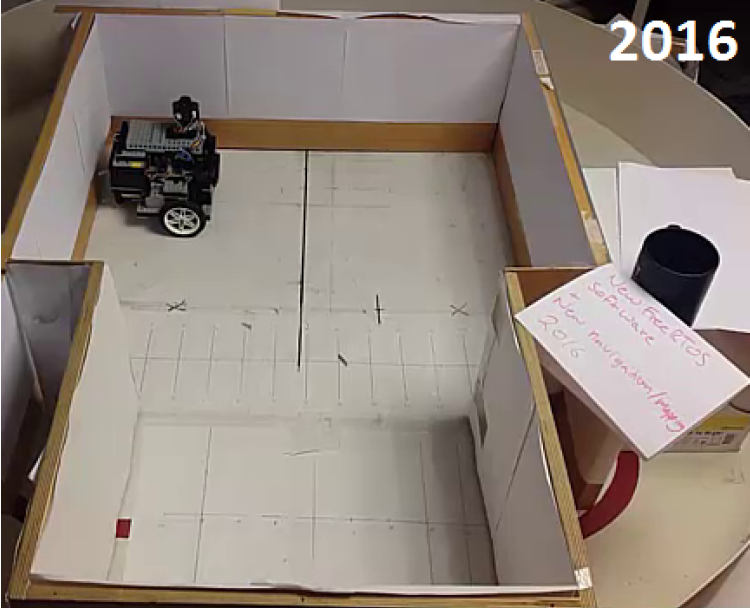
\includegraphics[width=0.8\textwidth]{fig/previous2}
  \caption{2016 Maze setup}
  \label{fig:previous2}
\end{figure}
\begin{figure}[H]
\centering
\includegraphics[width=0.4\textwidth]{fig/previous1}
  \caption{2016 AVR Robot Maze mapping result}
  \label{fig:previous1}
\end{figure}

% \begin{figure}[H]
% \centering
% 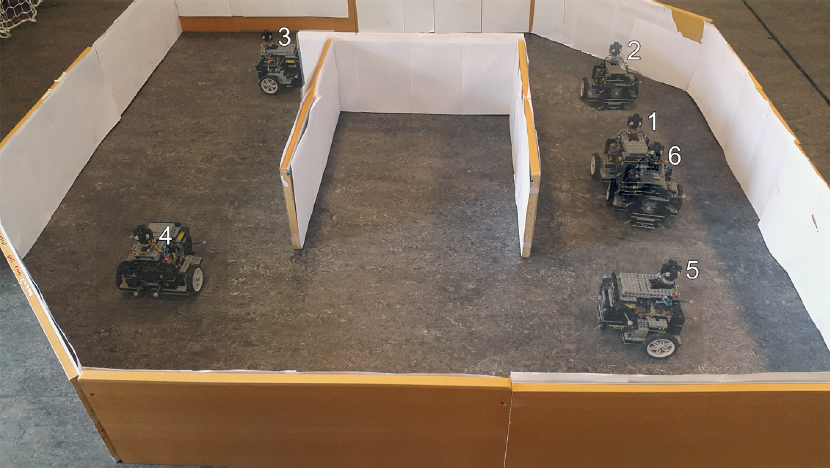
\includegraphics[width=1\textwidth]{fig/previous4}
%   \caption{Different Maze setup}
%   \label{fig:previous4}
% \end{figure}
% \begin{figure}[H]
% \centering
% 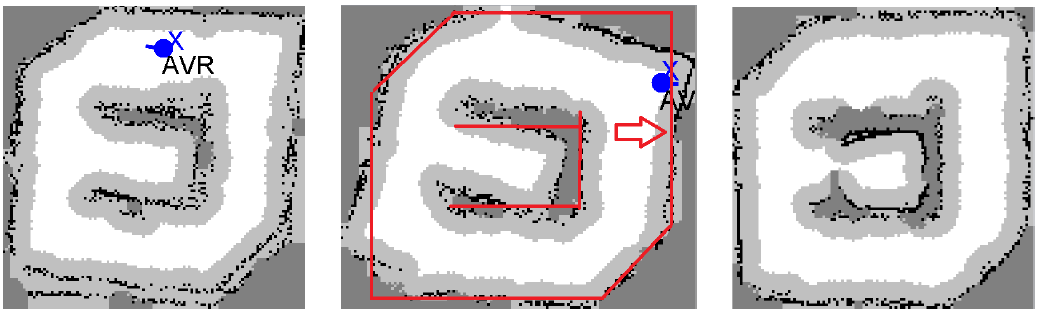
\includegraphics[width=1\textwidth]{fig/previous3}
%   \caption{Maze mapping result}
%   \label{fig:previous3}
% \end{figure}
These Figures were collected from Erlend Ese's masters thesis \cite{ese} from 2016.\\

\subsection{Accuracy}
\begin{figure}[H]
\centering
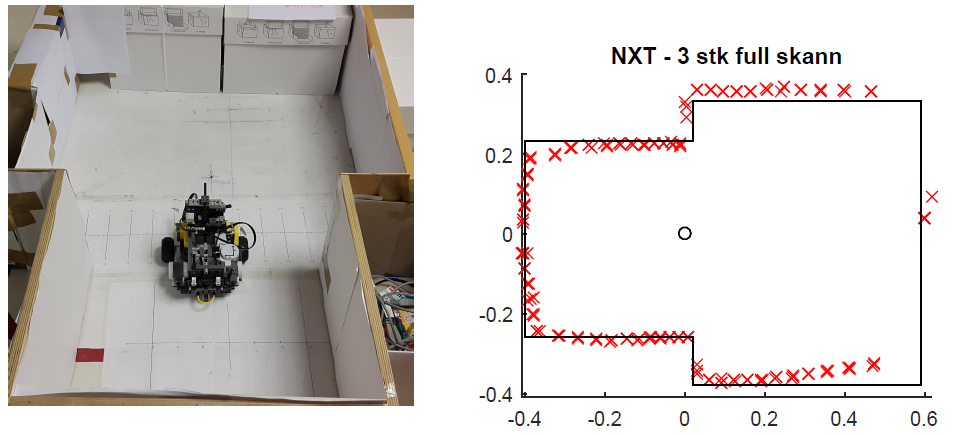
\includegraphics[width=\textwidth]{fig/previous5}
  \caption{2016 NXT Robot Maze mapping result}
  \label{fig:previous5}
\end{figure}
Looking at Figure \ref{fig:previous5} the real life maze setup has been plotted in the same plot as the estimated wall mapping. The mapping of the walls track the real life maze somewhat, but it curves at some points in the mapping, while at some points it does not even map the maze. The NXT Robot is only one of the different Lego-robots used for mapping. Figure \ref{fig:previous1} shows the AVR robot mapping, and this result is not a lot better than the NXT robot. \\

Comparing our mapping with the one from the AVR robot:
\begin{figure}[H]
\begin{subfigure}{.5\textwidth}
  \centering
  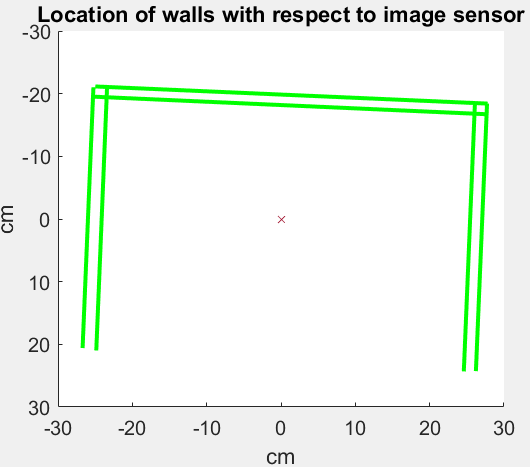
\includegraphics[width=\linewidth]{previous6}
  \caption{Bjørnsen}
\end{subfigure}
\begin{subfigure}{.5\textwidth}
  \centering
  \includegraphics[width=.9\linewidth]{previous1}
  \caption{Ese}
\end{subfigure}
\end{figure}
In terms of accuracy it is not easy to say something tangible, if it has improved with using an image sensor instead of the different sensors on the Lego robots. We know from our test on actual accuracy that my system could deliver an accuracy of $\pm0.5$ [cm], which might be an improvement over the older methods. On the other hand, this result might be too idealized and not applicable since the maze I mapped was not the same maze the Lego robots were tested on.\\

\subsection{Benefits of using an image sensor}
In the mazes I have tested on, the walls are straight. With this assumption, there are clear benefits of using an image sensor together with edge detection to map a maze, over the use of Lego robots. The implementation presented in this report will only detect straight wall segments, and therefor also represent them as straight walls:
\begin{figure}[H]
\begin{subfigure}{.5\textwidth}
  \centering
  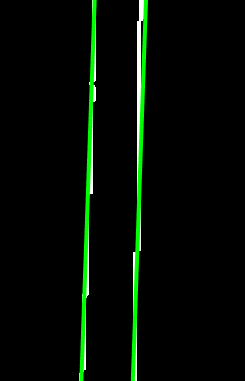
\includegraphics[width=.95\linewidth]{wall2}
  \caption{Wall detected in my report}
\end{subfigure}
\begin{subfigure}{.5\textwidth}
  \centering
  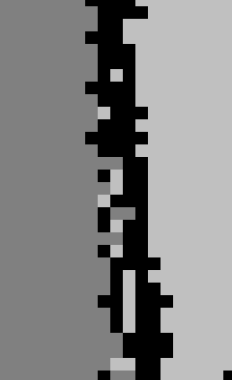
\includegraphics[width=.9\linewidth]{wall1}
  \caption{Same wall detected by Lego robots}
\end{subfigure}
\end{figure}

The walls detected by the Lego robots tend to be curved and are actually represented as a point cloud, and not as a vector in between two xy-coordinates.\\

\textbf{Improvements}
\begin{itemize}
\item Maps the maze characteristics as \emph{straight wall segments} in the real life xy-plane
\item Finer detailed
\item Not prone to accumulative estimator error the same way the Lego robots are
\end{itemize}













